\documentclass[tikz]{standalone}

\usetikzlibrary{positioning,calc}

\tikzset{
    pics/mig/.style = {
        code = {%
        \coordinate (-center) at (0, 0);
        \coordinate (-north) at (0, .5cm);
        \coordinate (-south) at (0,-.5cm);
        \coordinate (-se) at (310:.5cm);
        \coordinate (-sw) at (230:.5cm);
        \draw[line width=1mm](0,0)circle[radius=.5cm];
        }
    },
}
\begin{document}
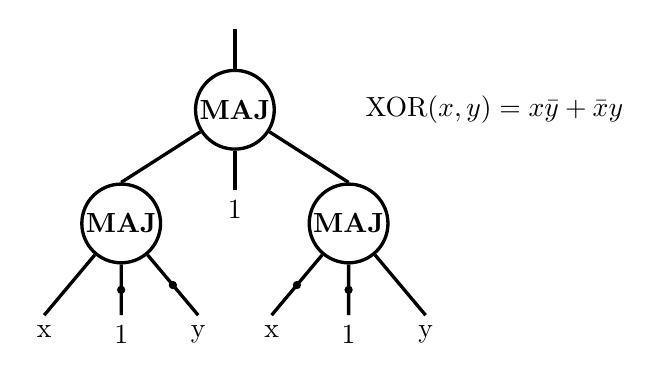
\begin{tikzpicture}[
    very thick,
    node distance = 1cm,
    mnode/.style={
        circle,
        draw, 
        inner sep=0pt, 
        minimum size=1cm
        },
    circ/.style={
        circle,
        fill,
        inner sep=0pt,
        minimum size=3pt,
        midway,
    },
]

\node[mnode](m1){\textbf{MAJ}};
\node[mnode, below left=of m1](m2){\textbf{MAJ}};
\node[mnode, below right=of m1](m3){\textbf{MAJ}};

\draw (m1.north) -- ++(0,.5cm);
\draw (m1.south) -- ++(0,-.5cm)node[below]{1};
\draw (m1) to (m2.north);
\draw (m1) to (m3.north);

\draw (m2.230) -- ++(230:1cm)coordinate(x2)node[below]{x};
\draw (m2.310) -- ++(310:1cm)coordinate(y2)node[below]{y}node[circ]{};
\draw (m2.south) -- ($(x2)!.5!(y2)$)node[circ]{}node[below]{1};

\draw (m3.230) -- ++(230:1cm)coordinate(x3)node[below]{x}node[circ]{};
\draw (m3.310) -- ++(310:1cm)coordinate(y3)node[below]{y};
\draw (m3.south) -- ($(x3)!.5!(y3)$)node[circ]{}node[below]{1};

\node[right=1cm of m1]{$\textrm{XOR}(x,y)=x\bar{y}+\bar{x}y$};

\end{tikzpicture}
\end{document}
